\chapter{Ergebnisse}

Zunächst testen wir, welche Art von Output sich für das Netz eignet. Dazu vergleichen wir die Performance unter Variation des Outputs mit den jeweils drei entsprechenden Datensätzen.

Anschließend integrieren wir das Netz in den DuckieTown-Simulator und bewerten die tatsächliche Performance.

\section{Wahl des Outputs}

\begin{figure}[H]
	\centering
	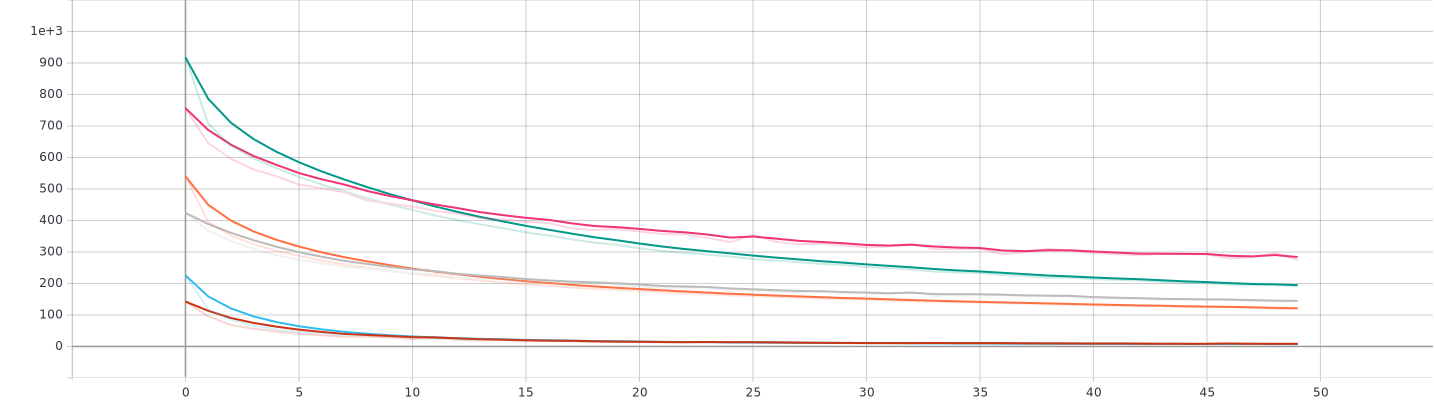
\includegraphics[width=\linewidth]{kapitel5/images//single-loss/Loss-single-loss.png}
	\caption{MSE mit 2D-Posenschätzung}
	\label{2d-poses-mse}
\end{figure}

\begin{figure}[H]
	\centering
	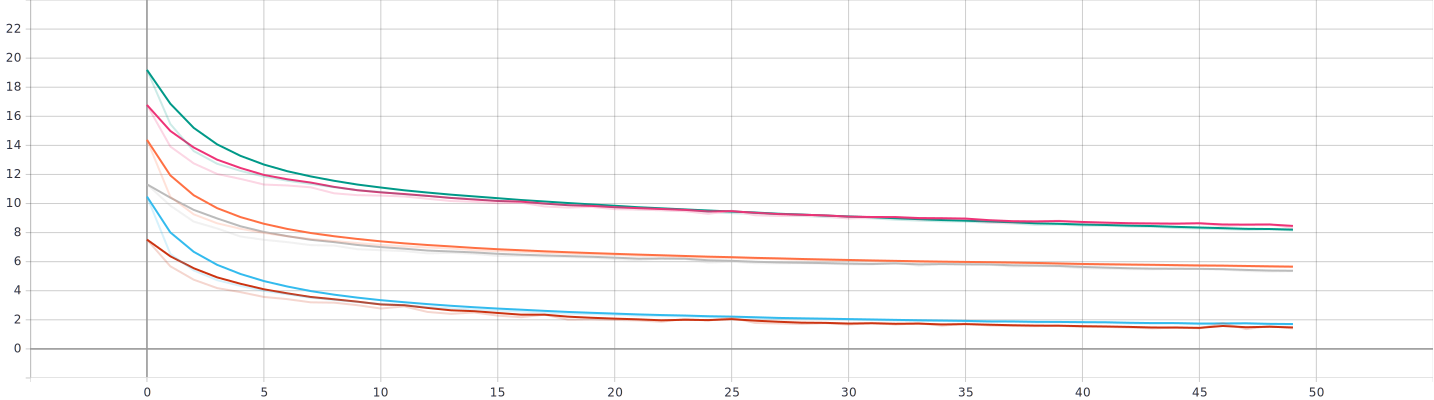
\includegraphics[width=\linewidth]{kapitel5/images/single-loss/Mean_Abs_Error_d-single-loss.png}
	\caption{MAE der Distanz mit 2D-Posenschätzung}
	\label{2d-poses-mae-d}
\end{figure}

\begin{figure}[H]
	\centering
	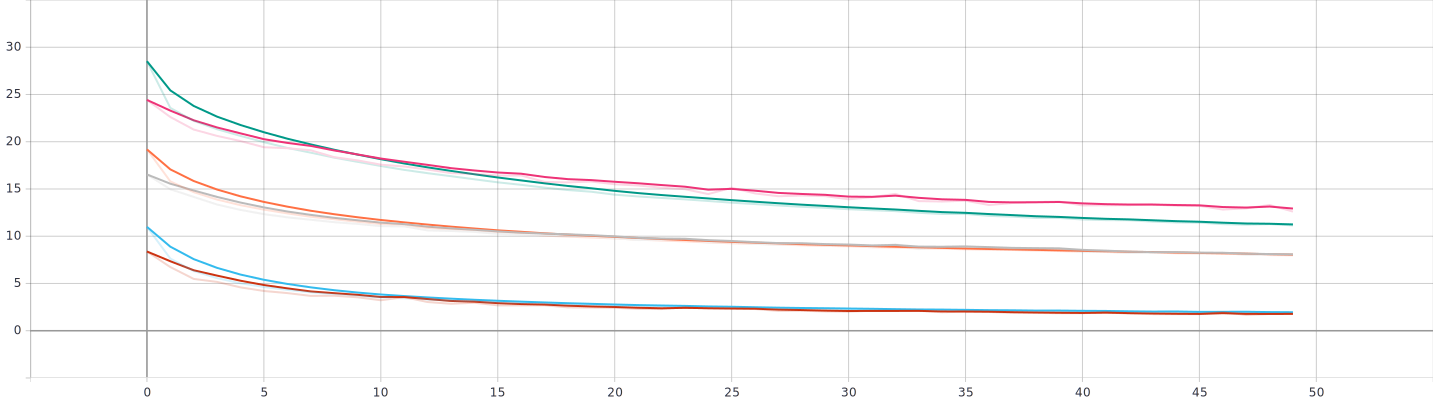
\includegraphics[width=\linewidth]{kapitel5/images/single-loss/Mean_Abs_Error_a-single-loss.png}
	\caption{MAE des Winkels mit 2D-Posenschätzung}
	\label{2d-poses-mae-a}
\end{figure}



\begin{figure}[H]
	\centering
	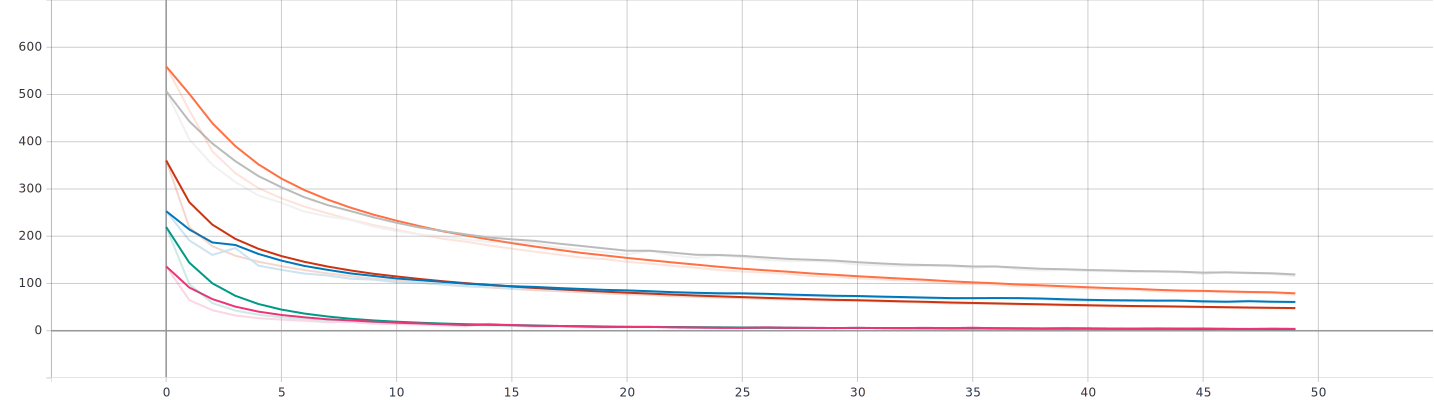
\includegraphics[width=\linewidth]{kapitel5/images/d-only/Loss-d-only.png}
	\caption{MSE der Distanz mit 1D-Posenschätzung}
	\label{1d-poses-mse-d}
\end{figure}

\begin{figure}[H]
	\centering
	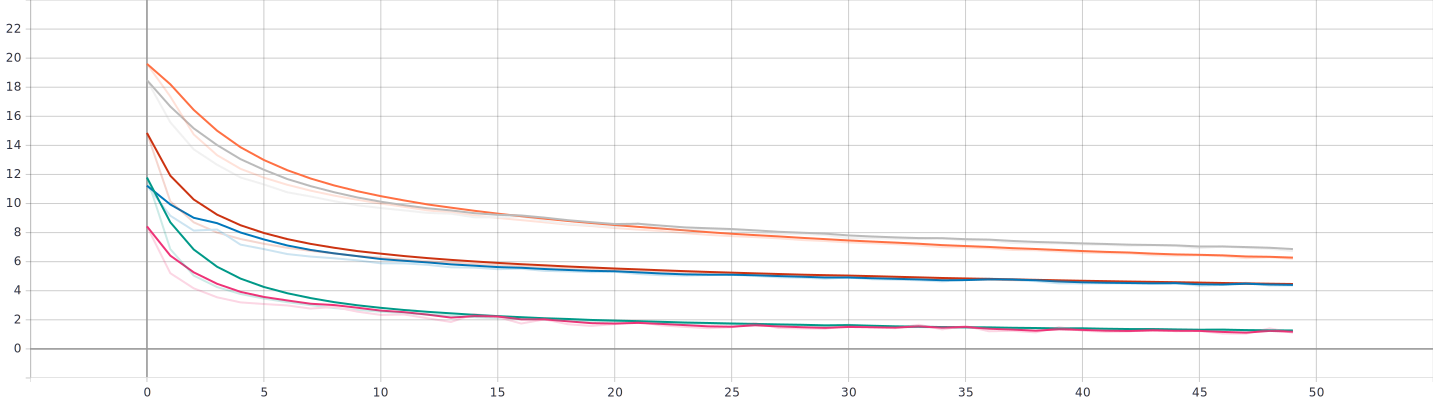
\includegraphics[width=\linewidth]{kapitel5/images/d-only/Mean_Abs_Error_d-d-only.png}
	\caption{MAE der Distanz mit 1D-Posenschätzung}
	\label{1d-poses-mae-d}
\end{figure}



\begin{figure}[H]
	\centering
	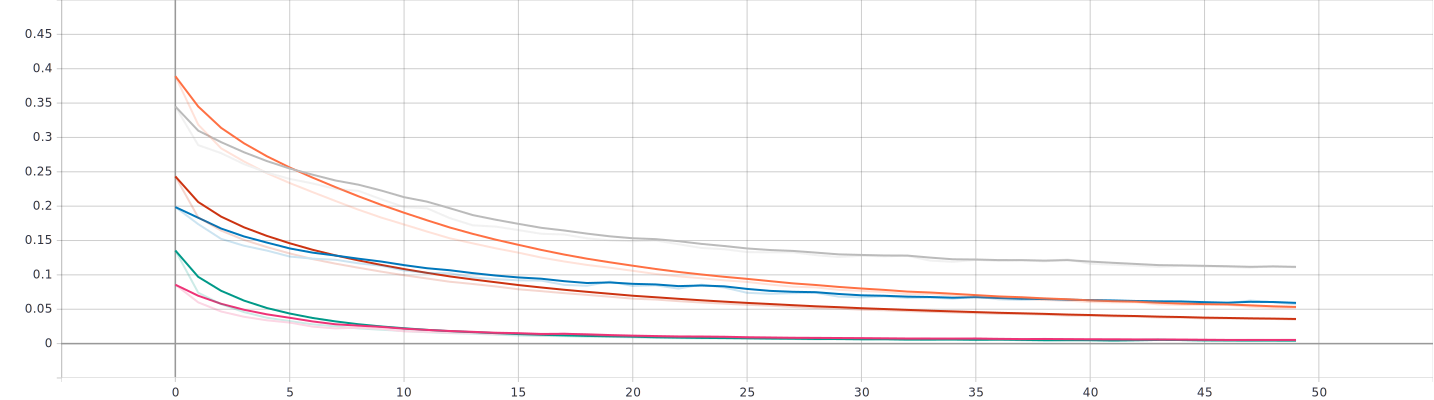
\includegraphics[width=\linewidth]{kapitel5/images/expert/Loss-expert.png}
	\caption{MSE der Winkelgeschwindigkeit mit Expertenbefehl}
	\label{expert-mse-omega}
\end{figure}

\begin{figure}[H]
	\centering
	\includegraphics[width=\linewidth]{kapitel5/images/expert/Mean_Abs_Error_omega-expert.png}
	\caption{MAE der Winkelgeschwindigkeit mit Expertenbefehl}
	\label{expert-mae-omega}
\end{figure}

\begin{tabular}[t]{|c|l|l|l|l|l|l|}
	\hline
	 & \textbf{Kacheltyp} & \textbf{mean} & \textbf{std} & \textbf{min} & \textbf{max} & \textbf{n} \\
	\hline
	\multirow{4}{*}{Datensatz 1} 
	& Alle & & & & & \\
	\cline{2-7}
	& Gerade & & & & & \\
	\cline{2-7}
	& Linkskurve & & & & & \\
	\cline{2-7}
	& 3-Wege-Kreuzung & & & & & \\
	\hline
	\multirow{4}{*}{Datensatz 2} 
	& Alle & & & & & \\
	\cline{2-7}
	& Gerade & & & & & \\
	\cline{2-7}
	& Linkskurve & & & & & \\
	\cline{2-7}
	& 3-Wege-Kreuzung & & & & & \\
	\hline
	\multirow{4}{*}{Datensatz 3} 
	& Alle & & & & & \\
	\cline{2-7}
	& Gerade & & & & & \\
	\cline{2-7}
	& Linkskurve & & & & & \\
	\cline{2-7}
	& 3-Wege-Kreuzung & & & & & \\
	\hline
\end{tabular}